%% This is the ctufit-thesis example file. It is used to produce theses
%% for submission to Czech Technical University, Faculty of Information Technology.
%%
%% Get the newest version from
%% https://gitlab.fit.cvut.cz/theses-templates/FITthesis-LaTeX
%%
%%
%% Copyright 2021, Eliska Sestakova and Ondrej Guth
%%
%% This work may be distributed and/or modified under the
%% conditions of the LaTeX Project Public Licenese, either version 1.3
%% of this license or (at your option) any later version.
%% The latest version of this license is in
%%  https://www.latex-project.org/lppl.txt
%% and version 1.3 or later is part of all distributions of LaTeX
%% version 2005/12/01 or later.
%%
%% This work has the LPPL maintenance status `maintained'.
%%
%% The current maintainer of this work is Ondrej Guth.
%% Contact ondrej.guth@fit.cvut.cz for bug reports.
%% Alternatively, submit bug reports into the tracker at
%% https://gitlab.fit.cvut.cz/theses-templates/FITthesis-LaTeX/issues
%%
%%

%%%%%%%%%%%%%%%%%%%%%%%%%%%%%%%%%%%%%%%%%
% CLASS OPTIONS
% language: czech/english/slovak
% thesis type: bachelor/master/dissertation
% colour: bw for black&white OR no option for default colour scheme
%%%%%%%%%%%%%%%%%%%%%%%%%%%%%%%%%%%%%%%%%
\documentclass[english,master,unicode]{ctufit-thesis}

%%%%%%%%%%%%%%%%%%%%%%%%%%%%%%%%%%
% FILL IN THIS INFORMATION
%%%%%%%%%%%%%%%%%%%%%%%%%%%%%%%%%%
\ctufittitle{Multiple target tracking with external information} % replace with the title of your thesis
\ctufitauthorfull{Bc. Andrey Babushkin} % replace with your full name (first name(s) and then family name(s) / surname(s)) including academic degrees
\ctufitauthorsurnames{Babushkin} % replace with your surname(s) / family name(s)
\ctufitauthorgivennames{Andrey} % replace with your first name(s) / given name(s)
\ctufitsupervisor{doc.\,Ing.\,Kamil Dedecius,\,Ph.D.} % replace with name of your supervisor/advisor (include academic degrees)
\ctufitdepartment{Department of Applied Mathematics} % replace with the department of your defence
\ctufityear{2023} % replace with the year of your defence
\ctufitdeclarationplace{Prague} % replace with the place where you sign the declaration
\ctufitdeclarationdate{\today} % replace with the date of signature of the declaration
\ctufitabstractCZE{Tato práce se zaměřuje na problém sledování více cílů v prostředí s vysokým množstvím rušení a nejistotou ohledně počtu sledovaných objektů pomocí Bayesovské inference. V této práci se hlavně zaměřujeme na populární Gaussian mixture probability hypothesis density (GM-PHD) filtr a představujeme techniku, jak zahrnout dodatečné informace pro případy, kdy senzor nedokáže detekovat sledované objekty z důvodu fyzických nebo prostředkových omezení. Poskytujeme veškeré potřebné teoretické pozadí od základů teorie pravděpodobnosti až po diskusi o různých metodách sledování více cílů a představení rámce Finite Set Statistics (FISST). Dále zahrnujeme rozsáhlé měření výkonnosti a analýzu výsledků, kde ukazujeme, že navržená technika fúze výrazně zlepšuje sledovací výsledky. Nakonec diskutujeme omezení filtru a navrhujeme možné způsoby, jak je překonat.
}
\ctufitabstractENG{The thesis focuses on the multi-target tracking problem in cluttered environments with the uncertainty on the number of targets and using Bayesian inference. In this work, we mainly focus on the popular Gaussian mixture probability hypothesis density (GM-PHD) filter and introduce a technique to include additional information for cases when a sensor fails to detect targets due to environmental or physical limitations. We provide all required theoretical background from the basics of probability theory to the discussion of various multi-target tracking methods and the introduction of the Finite Set Statistics (FISST) framework. We also conclude with an extensive performance measurement and analysis of results, where we demonstrate that the proposed fusion technique significantly improves tracking results. Finally, we discuss the limitations of the filter and propose possible measures to overcome them.
}
\ctufitkeywordsCZE{Bayesovské filtrování, sledování více cílů, náhodné množiny, gaussian mixture probability density filtr, fúze externích informací}
\ctufitkeywordsENG{Bayesian filtering, multi-target tracking, random finite sets, Gaussian Mixture Probability Density filter, external information fusion
}
%%%%%%%%%%%%%%%%%%%%%%%%%%%%%%%%%%
% END FILL IN
%%%%%%%%%%%%%%%%%%%%%%%%%%%%%%%%%%

%%%%%%%%%%%%%%%%%%%%%%%%%%%%%%%%%%
% CUSTOMIZATION of this template
% Skip this part or alter it if you know what you are doing.
%%%%%%%%%%%%%%%%%%%%%%%%%%%%%%%%%%

\RequirePackage{iftex}[2020/03/06]
\iftutex % XeLaTeX and LuaLaTeX
    \RequirePackage{ellipsis}[2020/05/22] %ellipsis workaround for XeLaTeX
\else
    \RequirePackage[utf8]{inputenc}[2018/08/11] %this file encoding
    \RequirePackage{lmodern}[2009/10/30] % vector flavor of Computer Modern font
\fi

% hyperlinks
\RequirePackage[pdfpagelayout=TwoPageRight,colorlinks=false,allcolors=decoration,pdfborder={0 0 0.1}]{hyperref}[2020-05-15]

% uncomment the following to hide all hyperlinks
% \RequirePackage[pdfpagelayout=TwoPageRight,hidelinks]{hyperref}[2020-05-15]

\RequirePackage{pdfpages}[2020/01/28]

\setcounter{secnumdepth}{4} % numbering sections; 4: subsubsection

%%%%%%%%%%%%%%%%%%%%%%%%%%%%%%%%%%
% CUSTOMIZATION of this template END
%%%%%%%%%%%%%%%%%%%%%%%%%%%%%%%%%%


%%%%%%%%%%%%%%%%%%%%%%
% DEMO CONTENTS SETTINGS
% You may choose to modify this part.
%%%%%%%%%%%%%%%%%%%%%%
\usepackage{dirtree}
\usepackage{lipsum,tikz}
\usepackage{csquotes}
\usepackage[style=iso-numeric]{biblatex}
\addbibresource{text/references.bib}
\usepackage{listings} % typesetting of sources
\usepackage{caption}
\usepackage{subcaption}  % subfigures
\usepackage{mathrsfs}  % mathscr
% \usepackage{minted} % typesetting of sources

%theorems, definitions, etc.
\theoremstyle{plain}
\newtheorem{theorem}{Theorem}
\newtheorem{lemma}[theorem]{Lemma}
\newtheorem{corollary}[theorem]{Corollary}
\newtheorem{proposition}[theorem]{Proposition}
\newtheorem{definition}[theorem]{Definition}
\theoremstyle{definition}
\newtheorem{example}[theorem]{Example}
\theoremstyle{remark}
\newtheorem{note}[theorem]{Note}
\newtheorem*{note*}{Note}
\newtheorem{remark}[theorem]{Remark}
\newtheorem*{remark*}{Remark}
\numberwithin{theorem}{chapter}
%theorems, definitions, etc. END
%%%%%%%%%%%%%%%%%%%%%%
% DEMO CONTENTS SETTINGS END
%%%%%%%%%%%%%%%%%%%%%%

\begin{document} 
\frontmatter\frontmatterinit % do not remove these two commands


\includepdf[pages={1-}]{assignment-include.pdf} % replace that file with your thesis assignment provided by study office

\thispagestyle{empty}\cleardoublepage\maketitle % do not remove these three commands

\imprintpage % do not remove this command

\tableofcontents % do not remove this command
%%%%%%%%%%%%%%%%%%%%%%
% list of other contents: figures, tables, code listings, algorithms, etc.
% add/remove commands accordingly
%%%%%%%%%%%%%%%%%%%%%%
\listoffigures % list of figures
\begingroup
\let\clearpage\relax
\listoftables % list of tables
\lstlistoflistings % list of source code listings generated by the listings package
% \listoflistings % list of source code listings generated by the minted package
\endgroup
%%%%%%%%%%%%%%%%%%%%%%
% list of other contents END
%%%%%%%%%%%%%%%%%%%%%%

\include{text/acknowledment}
%%%%%%%%%%%%%%%%%%%
% DECLARATION
% FILL IN / MODIFY
%%%%%%%%%%%%%%%%%%%
% INSTRUCTIONS
% ENG: choose one of approved texts of the declaration. DO NOT CREATE YOUR OWN. Find the approved texts at https://courses.fit.cvut.cz/SFE/download/index.html#_documents (document Declaration for FT in English)
% CZE/SLO: Vyberte jedno z fakultou schvalenych prohlaseni. NEVKLADEJTE VLASTNI TEXT. Schvalena prohlaseni najdete zde: https://courses.fit.cvut.cz/SZZ/dokumenty/index.html#_dokumenty (prohlášení do ZP)
\begin{declarationpage}
I hereby declare that the presented thesis is my own work and that I have cited all sources of information in accordance with the Guideline for adhering to ethical principles when elaborating an academic final thesis.

I acknowledge that my thesis is subject to the rights and obligations stipulated by the Act No. 121/2000 Coll., the Copyright Act, as amended, in particular that the Czech Technical University in Prague has the right to conclude a license agreement on the utilization of this thesis as a school work under the provisions of Article 60 (1) of the Act.
\end{declarationpage}
%%%%%%%%%%%%%%%%%%%
% DECLARATION END
%%%%%%%%%%%%%%%%%%%

\printabstractpage % do not remove this command
%%%%%%%%%%%%%%%%%%%
% SUMMARY
% FILL IN / MODIFY
% OR REMOVE ENTIRELY (upon agreement with your supervisor)
% (appropriate to remove in most theses)
%%%%%%%%%%%%%%%%%%%
\begin{summarypage}
\section*{Summary section}

\lipsum[1][1-8]

\section*{Summary section}

\lipsum[2][1-6]

\section*{Summary section}

\lipsum[3]

\section*{Summary section}

\lipsum[2]

\section*{Summary section}

\lipsum[1][1-8] Lorem lorem lorem.
\end{summarypage}
%%%%%%%%%%%%%%%%%%%
% SUMMARY END
%%%%%%%%%%%%%%%%%%%

%%%%%%%%%%%%%%%%%%%
% ABBREVIATIONS
% FILL IN / MODIFY
% OR REMOVE ENTIRELY
% List the abbreviations in lexicography order.
%%%%%%%%%%%%%%%%%%%
\chapter{List of Acronyms}

\begin{tabular}{rl}
CV & Constant Velocity \\
EKF & Extended Kalman filter \\
FISST & Finite Set Statistics \\
FoV & Field of view \\
GM & Gaussian mixture \\
HO-MHT & Hypothesis-oriented Multiple Hypothesis Tracker \\
JPDA & Joint Probabilistic Data Association \\
KF & Kalman filter \\
MAP & Maximum a posteriori \\
MHT & Multiple Hypothesis Tracker \\
MLE & Maximum Likelihood Estimator \\
MMSE & Minimum Mean Square Error \\
MTT & Multitarget tracking \\
PDA & Probabilistic Data Association \\
PHD & Probability hypothesis density \\
PPP & Poisson Point Process \\
RFS & Random Finite Set \\
TO-MHT & Track-oriented Multiple Hypothesis Tracker \\
UKF & Unscented Kalman Filter \\
\end{tabular}
%%%%%%%%%%%%%%%%%%%
% ABBREVIATIONS END
%%%%%%%%%%%%%%%%%%%


%%%%%%%%%%%%%%%%%%%
% THE THESIS
% MODIFY ANYTHING BELOW THIS LINE
%%%%%%%%%%%%%%%%%%%
\graphicspath{figures}
\mainmatter\mainmatterinit % do not remove these two commands

%%%%%%%%%%%%%%%%%%%%%%%%%%%%%%%%%%%%%%%%%%
% Introduction
%%%%%%%%%%%%%%%%%%%%%%%%%%%%%%%%%%%%%%%%%%
\addcontentsline{toc}{chapter}{Introduction}\markboth{Introduction}{Introduction}
\setcounter{page}{1}

\chapter*{Introduction}Object tracking is a critical problem in signal processing and computer vision. The primary goal of tracking algorithms is to estimate the states of moving targets based on a sequence of sensor measurements in environments with a high degree of uncertainty. Different domains of the problem require different approaches to target tracking. In this work, we provide an overview of the existing areas of target tracking and introduce the scope of this study.

Tracking algorithms can be categorized based on the number of targets they track, whether it is a fixed or known number of targets, or a variable and unknown number of targets. When the number of targets in the tracking area is greater than one, we refer to it as multi-target tracking (MTT). Object tracking is widely used in various fields, including robotics, autonomous vehicles, surveillance, and medical imaging. With the recent emergence of deep learning algorithms, there has been renewed interest in MTT, and many new deep learning-based approaches have been proposed. However, the learned model's predictive power is questionable, as these approaches estimate the internal object dynamics using complex non-linear models, while the Bayesian approach assumes fixed known model that are specified manually according to some prior knowledge, for instance, physical laws. In this study, we focus on MTT using Bayesian inference, the statistical approach based on recursive updates of the target posterior distribution using a set of measurements.

Bayesian algorithms are classified based on the results they achieve \cite[11]{sarkkaBayesianFilteringSmoothing2013}. The first type of algorithms is Bayesian smoothers, which remove the noise of states based on past and future measurements, i.e., they smooth the signal. The other type is Bayesian predictors, which predict the future state of a target more than one step ahead based on past measurements. The last type is Bayesian filters, which predict the current state of a target based on measurements up to the moment of the predicted state. The Kalman filter, the fundamental algorithm for many modern and sophisticated tracking methods, is an example of Bayesian filters. This study focuses on Bayesian filters, and we cover the Kalman filter in detail.

Algorithms can also be separated based on the type of sensor and measurements used. There are several sets of algorithms available to address specific problems depending on the sensors used. For instance, point object tracking is used when the sensor generates one measurement per object, such as a radar or a camera with an object recognition algorithm. When lidars are used, one target generates a set of measurements, and this is referred to as extended object tracking \cite{granstromExtendedObjectTracking2017}. In surveillance, especially when tracking people, group object tracking algorithms are used to estimate groups of individuals rather than every individual separately \cite{salmondGroupExtendedObject1999}. Additionally, tracking with multipath propagation refers to scenarios where a sensor receives more than one detection caused by the multipath phenomenon or multiple reflections from surrounding objects of the same signal \cite{bar-shalomTrackingLowElevation1994}. Finally, tracking with unresolved targets occurs when several targets produce only one measurement \cite{angleMultipleTargetTracking2021}. In this study, we focus on point object tracking, assuming that one target produces at most one measurement, and each measurement can be generated by at most one target.

This study aims to enhance the performance of the Gaussian Mixture probability hypothesis density (GM-PHD) filter, a popular Bayesian filter for multi-target tracking (MTT), by proposing a novel approach to incorporate external information. Specifically, we provide a detailed description of the GM-PHD filter and its internals, and demonstrate through an example how the filter may fail under environmental limitations. We then introduce our proposed method for integrating external information and analyze its impact on the filter's performance. Finally, we evaluate the filter's strengths and weaknesses in various scenarios and discuss the significance of our contribution in improving the accuracy and robustness of the GM-PHD filter for MTT.

\section*{Motivation}% Motivation of this work
% main questions and goals

\section*{Related works}% Previous research on object tracking
% different Bayesian filters, GM-PHD, etc.

\section*{Contribution of this work}% Contribution of the work
\section*{Structure}The thesis is structured as follows. Chapter 1 provides the theoretical background necessary for understanding the rest of the thesis, including the introduction of probability theory and probability distributions and the Bayes' rule. Next, we present the Bayesian inference framework, which is the basis for the general Bayes filter, a recursive algorithm for state estimation. Finally, we present the concepts of state-space models and the Kalman filter.

Chapter 2 is dedicated to multi-target tracking. It starts with an overview of target tracking methods, followed by an introduction to Random Finite Sets (RFS). The chapter then describes the PHD filter and the PHD function. Next, we give a PHD filter formal definition, and then observe the Gaussian Mixture PHD filter. The chapter concludes with a discussion of track maintenance, the GM-PHD recursion, and ends with the framework for external information fusion.

Chapter 3 describes the implementation and testing methodology of the GM-PHD filter. We then introduce several metrics that are used to measure the performance of multi-target tracking algorithms, then we describe four testing scenarios. The final section on parameters testing and methodology explains how the tests were conducted and how the results were analyzed.

Chapter 4 analyzes the results of the tests conducted in Chapter 3. This chapter includes sections on test results for each scenario and a discussion of the results, where a comprehensive analysis of the filter strengths and weaknesses is provided.

The final Chapter 5 concludes this work by summarizing the main contributions of the thesis and highlighting areas for future research.


%%%%%%%%%%%%%%%%%%%%%%%%%%%%%%%%%%%%%%%%%%
% Theoretical background
%%%%%%%%%%%%%%%%%%%%%%%%%%%%%%%%%%%%%%%%%%
\chapter{Theoretical background}The field of target tracking, both single and multiple, rely on mathematical concepts and methods based on probability theory. In this chapter, we provide an introduction to key concepts of probability and inference. We start by reviewing the basics of probability theory, including random variables, probability distributions with examples of the most important ones for multi-target tracking, and the Bayes' theorem. Then, we describe the concept of state-space models, a powerful framework that allows to describe dynamic system evolving in time. Then, we apply these concepts with a Bayes filter, a general method for recursive estimation the state of a dynamic system using measurements obtained from a sensor over time. Finally, we define and prove two important in tracking theorems, and use these theorems to derive the Kalman filter, and important and widely used framework that provides an optimal state estimate of a linear system in the presence of Gaussian noise. The theoretical foundations in this chapter serve as a basis for the next chapter, which covers more sophisticated algorithms for tracking multiple targets in noisy environments.

\section{Probability theory foundations}% Introduction to probability theory
    % - [x] Basic concepts such as events, outcomes, and sample spaces
    % - [x] Definition of probability and probability axioms
    % - [x] Definition of conditional probability
    % - [x] Bayes' rule and its derivation
    % - [x] Discrete and continuous probability distributions
    % - [x] Expectation, variance, and covariance
    % - [x] Known probability distributions and their properties

\renewcommand{\Pr}[1]{\operatorname{Pr}\{#1\}}

When we are dealing with probability of an event, we assume that there is a possibility
of that event occurring and we measure it using a number between 0 and 1 or a percentage
between 0\% and 100\%. In other words, we use the probability theory framework to assign
numerical values to arbitrary events. This section covers several fundamental concepts of
probability theory, which serve as the basis for this work.

The \textit{event}, which we formally denote as $E$, comes from some space of all possible
events, the \textit{outcome space} $\Omega$. We also denote the \textit{probability} of the
event $E$ as $\Pr{E}$. This probability is a real non-negative number,
that is $\Pr{E} \in \mathbb{R}, \Pr{E} \geq 0$. The outcome
space covers all possible events, that is $\Pr{\Omega} = 1$. It then follows
that the probability of disjoint events from the outcome space $\Omega$ is the sum of
probabilities of these events, that is for
$E_1, \ldots, E_n \in \Omega, \Pr{\bigcup_{i=1}^n E_i} = \sum_{i=1}^n \Pr{E_i}$.

We have defined three main axioms of probability theory. In addition to these axioms, several
crucial concepts illustrate the relationship between events. Given two events, $E_1$ and $E_2$,
the \textit{conditional probability} of $E_1$ given $E_2$ is defined as

$$
\Pr{E_1 \mid E_2} = \frac{\Pr{E_1 \cap E_2}}{\Pr{E_2}}.
$$

If the events are \textit{independent} of each other, the probability of them occurring
simultaneously is given by

$$
\Pr{E_1 \cap E_2} = \Pr{E_1}\Pr{E_2}.
$$

These relationships allow us to define the \textit{law of total probability}
\cite[31]{zwillingerCRCStandardProbability2000}, which is a key component of Bayes' rule.
Let $A$ be an event, $A \int \Omega$, and $\{B_n : n = 1, 2, \ldots\}$ be a countable
partition of the space $\Omega$. Then, we have:

$$
\Pr{A} = \sum_n \Pr{A \mid B_n} \Pr{B_n}.
$$

Now, we can deduce the following rule:

\begin{definition}[Bayes' rule]
Let $A$ and $B$ be two events from the outcome space $\Omega$. Then the following applies:

$$
\Pr{A \mid B} = \frac{\Pr{B \mid A}}{\Pr{B}}
    = \frac{\Pr{B \mid A}}{\sum_n \Pr{B \mid A_n}\Pr{A_n}}.
$$
\end{definition}

Bayes' rule plays a crucial role in Bayesian inference and serves as the basis for
Bayesian filters, including the PHD filter.

\subsection{Probability distributions}

Events and their probabilities are not sufficient for our purposes;
we need a framework that allows us to obtain a formal, general description of a set
of events from some outcome space. Specifically, we need an abstraction around events,
which is some function that maps the outcome space $\Omega$ to some other space,
typically $\mathbb{R}$ (but not necessarily). This abstraction is called a
\textit{random variable} and one outcome of it is called a \textit{realization}.

\begin{definition}[Random variable and its realization]
    Let $\Omega$ be a set of possible events, $\omega \in \Omega$ is some event,
    and $\mathbb{O}$ be another space. A function $X: \Omega \rightarrow \mathbb{O}$
    is called a random variable and $x = X(\omega)$ is called a realization of $X$.
\end{definition}

The above definition provides a general framework for understanding random variables.
However, for the purposes of Bayesian statistics, we will simplify the discussion by
focusing on scalar, continuous-valued random variables, represented
by $\mathbb{O} = \mathbb{R}$. In practice, it is often impractical to calculate the
probability of every possible event from the outcome space $\Omega$, especially for
continuous random variables with uncountably infinite outcomes. Instead, it may suffice
to work with intervals on the outcome space and their probabilities. We call such a
probability distribution a \textit{cumulative distribution function (cdf)} of $X$,
and the first-order derivative of the cdf is called a \textit{probability density
function (pdf)}.\footnote{
    For discrete random variables, the corresponding distribution function is
    called a \textit{probability mass function (pmf)}.
}

\begin{definition}[Cumulative distribution function (cdf)]
    Given a scalar real-valued random variable $X \in \mathbb{R}$ and $x$ as a
    realization of $X$, we define the probability $\Pr{X \in (-\infty, x)} = \Pr{X < x}$
    as the cumulative distribution function of random variable $X$ and denote it as $P(x)$.
\end{definition}

\begin{definition}[Probability density function (pdf)]
    The probability density function $p(x)$ of a scalar real-valued random variable $X$
    is defined as:
    $$
    p(x) = \frac{\partial P(x)}{\partial x}.
    $$
\end{definition}

Probability distributions are fundamental in Bayesian statistics and provide a way
to model and analyze the behavior of random variables. In the next section,
we will discuss some common probability distributions used in Bayesian filters,
including the Gaussian distribution and the Poisson distribution.

Probability distributions are fundamental in Bayesian statistics and provide a way
to model and analyze the behavior of random variables. Cdfs and pdfs (as well as pmfs
for discrete cases) are used to specify the probability distribution of a random
variable, providing a formal description of the relationship
between events and probabilities. In addition to this formal description, we also
need to know several statistical properties of probability distributions to fully
understand their behavior. Two main properties of probability distributions are
the expected value, $E[X]$, and the variance, $\operatorname{Var}[X]$:

$$
\begin{aligned}
E[X]&=\int_{-\infty}^{\infty} x p(x) d x \\
\operatorname{Var}[X]
    &= E\left[(X-E[X])^2\right]
    =\int_{-\infty}^{\infty}(x-E[X])^2 p(x) d x.
\end{aligned}
$$

The expected value, or the first moment, represents the most probable value of
a random variable. The variance, or the second central moment, is a measure of the
variability of a random variable and is often denoted as $\operatorname{Var}[X] = \sigma^2$.
Furthermore, we often study the relationship between two random variables, say $X$ and
$Y$, and measure their joint variability, which we call a \textit{covariance}:

$$
\operatorname{Cov}[X, Y]
    = E\left[(X-E[X])(Y-E[Y])\right]
    =\int_{-\infty}^{\infty}(x-E[X])(y-E[Y]) p(x, y) d x d x.
$$

For vector-valued random variables, that is $X, Y \in \mathbb{R}^k$ and $\mathbf{x}$
is the realization of $X$, the formulas are the following. It is worth noting that
the covariance in the vector case becomes a matrix and is called a \textit{covariance
matrix}:

$$
\begin{aligned}
E[X]
    &=\int_{-\infty}^{\infty} \mathbf{x} p(\mathbf{x}) d \mathbf{x} \\
\operatorname{Var}(X)
    &= E\left[\left(X-E[X]\right)\left(X-E[X]\right)^\intercal\right]
    \\&=\int_{-\infty}^{\infty}
        \left(\mathbf{x}-E[X]\right)
        \left(\mathbf{x}-E[X]\right)^\intercal
        p(\mathbf{x})
        d \mathbf{x} \\
\operatorname{Cov}[X, Y]
    &= E\left[\left(X-E[X]\right)\left(Y-E[Y]\right)^\intercal\right]
    \\&=\int_{-\infty}^{\infty}
        \left(\mathbf{x}-E[X]\right)
        \left(\mathbf{y}-E[Y]\right)^\intercal
        p(\mathbf{x}, \mathbf{y})
        d \mathbf{x} d \mathbf{y}.
\end{aligned}
$$

Probability distributions are fundamental in Bayesian statistics and
provide a way to model and analyze the behavior of random variables. For
the purpose of Bayesian filters, some common probability distributions
are particularly useful. In this section, we will discuss some of these
distributions and their main properties. We shall start from discrete
cases and go on to the continuous variables.  % uniform, bernoulli, poisson, gaussian

\subsubsection{Bernoulli distribution}

The Bernoulli distribution is the simplest discrete probability
distribution, and the Bernoulli random variable is binary, with only
two realizations, $0$ or $1$. This distribution is parameterized with 
$r$, the probability of the positive outcome. Its probability mass 
function is given by

$$
p(x) = \begin{cases}
 1 - r, & \text{if } x = 0, \\
     r, & \text{if } x = 1, \\
     0, & \text{otherwise}.
\end{cases}
$$

\begin{figure}
\centering
\begin{subfigure}{.5\textwidth}
  \centering
  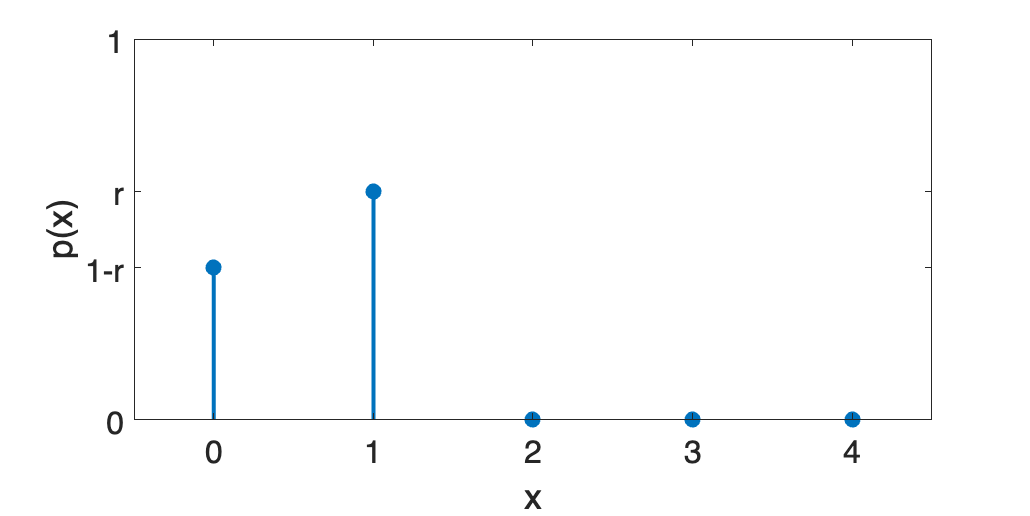
\includegraphics[width=.9\linewidth]{figures/bern.pmf.png}
  \caption{PMF.}
  \label{fig:bern:pmf}
\end{subfigure}%
\begin{subfigure}{.5\textwidth}
  \centering
  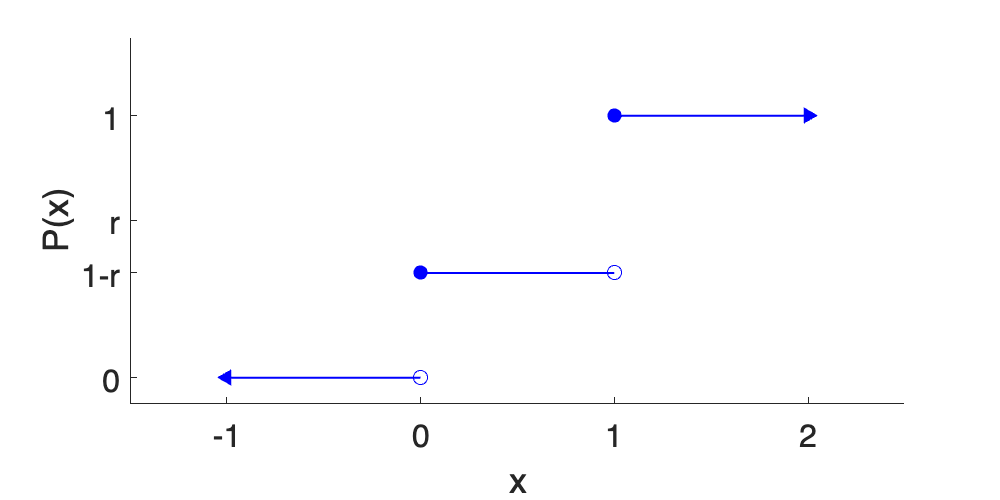
\includegraphics[width=.9\linewidth]{figures/bern.cdf.png}
  \caption{CDF.}
  \label{fig:bern:cdf}
\end{subfigure}
\caption{Bernoulli distribution.}
\label{fig:bern}
\end{figure}

The pmf and the cdf of the Bernoulli distribution can be seen on Figure \ref{fig:bern}.
We denote this distribution as $p(x) = \operatorname{Bernoulli}(x;r)$.
The expected value and the covariance of a Bernoulli random variable $X$ are

$$
E[X] = r, \qquad \operatorname{Var}[X] = r(1-r).
$$

In object tracking, we use Bernoulli random variables to model the existence of
an object at some time step $k$, which we will discuss in detail in the following
sections.

\subsubsection{Binomial distribution}

Binomial random variables are the generalization of Bernoulli random variables,
representing the probability of $x$ positive outcomes after $n$ consecutive and
independent trials. This distribution is parameterized by the probability of the
positive outcome in one trial $r$ and the number of trials $n$. Its pmf, as well 
as the expected value and the variance, are given by

$$
\begin{aligned}
    p(x) &= \binom{n}{x} r^x (1-r)^{(n-x)}, \\
    E[X] &= nr, \\
    \operatorname{Var}[X] &= nr(1-r).
\end{aligned}
$$

\subsubsection{Poisson distribution}

The Poisson distribution is a discrete random distribution that can 
be used as an approximation of the Binomial distribution in cases where 
$n$ tends towards infinity and $r$ tends towards $0$ such that their 
product stays about equal to a parameter $\lambda$, which is the 
parameter of the Poisson distribution and also its expected value and 
variance. The outcome space of a Poisson random variable is 
$\mathbb{N}_0$,\footnote{Natural numbers including $0$.} and its pmf,
expected value and variance are given by

$$
\begin{aligned}
    p(x) = \operatorname{Poisson}(x; \lambda) &= \frac{\lambda^x e^{-\lambda}}{x !}, \\
    E[X] = \operatorname{Var}[X] &= \lambda.
\end{aligned}
$$

The probability mass function and the corresponding cumulative density functions
of the Poisson distribution can be seen in Figure \ref{fig:poisson}.
The Poisson distribution is a critical component of modern multi-object
tracking systems, as it is used to model noise measurements, and some 
systems even use it to model objects that exist but are not visible in
the field of view of a sensor \cite{garcia-fernandezPoissonMultiBernoulliMixture2018}.
The Poisson distribution is the foundation of the so-called Poisson Point
Processes (PPP), which will be discussed later.

\begin{figure}
\centering
\begin{subfigure}{.5\textwidth}
  \centering
  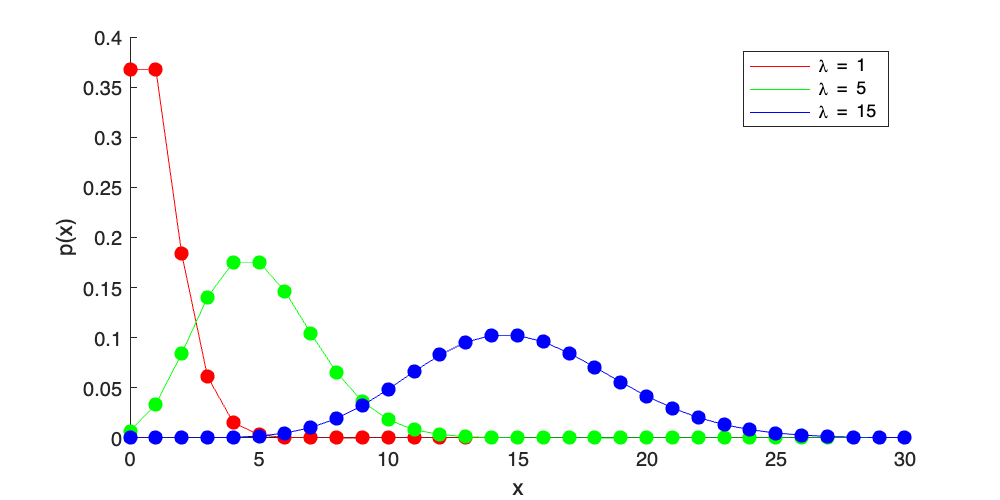
\includegraphics[width=.9\linewidth]{figures/poisson.pmf.png}
  \caption{PMF.}
  \label{fig:poisson:pmf}
\end{subfigure}%
\begin{subfigure}{.5\textwidth}
  \centering
  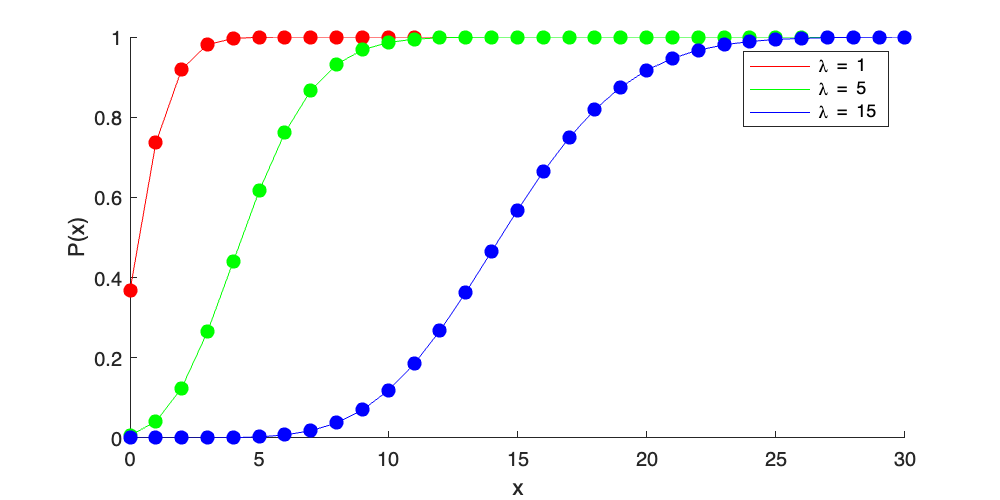
\includegraphics[width=.9\linewidth]{figures/poisson.cdf.png}
  \caption{CDF.}
  \label{fig:poisson:cdf}
\end{subfigure}
\caption{Poisson distribution.}
\label{fig:poisson}
\end{figure}

\subsubsection{Uniform distribution}

The uniform distribution is a continuous probability distribution and it
describes such random variables which outcomes on some interval $[a, b]$
are possible with equal probability. This distribution is parameterized by
$a$ and $b$ and its pdf, $E[X]$ and $\operatorname{Var}[X]$ are:

$$
\begin{aligned}
    p(x)
        =\operatorname{Uniform}(x; [a, b])
        &= \begin{cases}
            \frac{1}{b-a} & \text { if } a \leq x \leq b, \\
            0 & \text { otherwise, }
        \end{cases} \\
    E[X] &= \frac{a + b}{2}, \\
    \operatorname{Var}[X] &= \frac{(b - a)^2}{12}.
\end{aligned}
$$

The uniform distribution is generally used to represent the uncertainty when
all outcomes are equally possible. In this work, we use the uniform distribution
to model positions of clutter measurements at some time step $k$.

\subsubsection{Gaussian distribution}

The Gaussian distribution, also known as the normal distribution, is a 
continuous probability distribution that is widely used in many branches
of statistics, including Bayesian filtering. It is typically used to model
a large number of independent and identically distributed (i.i.d.) random variables.

The Gaussian distribution is characterized by two parameters: the mean 
$\mu$ and the variance $\sigma^2$. Its probability density function (pdf), 
expected value, and variance are given by:

$$
\begin{aligned}
    p(x)
        =\mathscr{N}\left(x ; \mu, \sigma^2\right)
        &=\frac{1}{\sqrt{2 \pi} \sigma} \exp \left(\frac{(x-\mu)^2}{2 \sigma^2}\right), \\
    E[X] &= \mu, \\
    \operatorname{Var}[X] &= \sigma^2.
\end{aligned}
$$

Despite not having a closed-form solution, the Gaussian distribution 
possesses several desirable properties that allow for closed-form solutions 
in many applications, including object tracking. Although it may be too 
simple to model certain scenarios, it represents the approximate average 
position of objects and their uncertainty quite well. This work utilizes
mixtures of Gaussians, which will be discussed in more detail later.


% - Probability theory, Bayes' rule, Bayesian inference, likelihood
% - State-space model
% - Kalman filter
% - Constant velocity model (incl. the measurement model, which is a part of CVM)
% - Multi-object tracking problem, assumptions
%     - Recall some part from Intro, gradually from JPDA to PHD
% - Object birth/survival
% - PHD filter
% - GM-PHD filter
% - Inclusion of external information, Gaussian fusion
%     - Known stuff is gone, new stuff's coming
% - Convergence analysis?

%%%%%%%%%%%%%%%%%%%%%%%%%%%%%%%%%%%%%%%%%%
% Implementation and testing
%%%%%%%%%%%%%%%%%%%%%%%%%%%%%%%%%%%%%%%%%%
\chapter{Implementation and tests}This chapter presents the methodology we used to test the performance of the GM-PHD filter. Firstly, we introduce two metrics that are appropriate for use in measuring the performance of a multi-target tracking algorithm. Secondly, we describe in detail several test scenarios on which the testing was conducted. Finally, we explain the ranges of different initial settings that were tested and describe the implementation of the GM-PHD filter.

% - Implementation overview
% - GM-PHD algorithm, Python implementation description
% - Test scenarios, data generation
% - Metrics: CPEP, EAE

%%%%%%%%%%%%%%%%%%%%%%%%%%%%%%%%%%%%%%%%%%
% Results analysis
%%%%%%%%%%%%%%%%%%%%%%%%%%%%%%%%%%%%%%%%%%
\chapter{Results analysis}In this chapter, we present the results of a thorough testing of different parameters of the GM-PHD filter on different test cases presented in the previous chapter. For convenience, we have split this chapter into multiple sections, referring to each test scenario and included multiple plots that depict the change of both the CPEP metric and the expected absolute error on the number of targets. Finally, we discuss the results, outline the strengths and weaknesses of the GM-PHD filter, and compare the results of the (C3) and (C4) scenarios, with and without external information fusion.

% - Results obtained from tests, graphs
% - Comparison GM-PHD vs. GM-PHD with externals information
% - Change of performace due to changes of different parameters
% - Quantitative and qualitative evaluation of results
% - Tracks and observed problems
% - Discussion on the performance evaluation
% - Limitations

%%%%%%%%%%%%%%%%%%%%%%%%%%%%%%%%%%%%%%%%%%
% Conclusion
%%%%%%%%%%%%%%%%%%%%%%%%%%%%%%%%%%%%%%%%%%
\chapter{Conclusion}In this work, we explored one of the most popular Bayesian filters for multi-target tracking in Gaussian-linear cases, the Gaussian Mixture Probability Density (GM-PHD) filter. We investigated its performance and robustness in several tracking scenarios, including challenging situations where a sensor fails to collect measurements from targets and external information fusion is required.

We have demonstrated that the performance of the GM-PHD filter can be improved by incorporating external estimates from other sensors, as shown through evaluation of several metrics that indicated significant improvement in tracking results.

However, we have also identified a problem with track continuity when using the simple tagging of Gaussian components. We believe that more sophisticated techniques may improve track maintenance of the GM-PHD filter and make it more robust to complex scenarios with high uncertainty due to clutter measurements and a high number of targets.

Additionally, we have measured and discussed the filter's performance depending on the setup of internal parameters. We observed that the GM-PHD filter was sensitive to the choice of settings, particularly the clutter rate and probability of detection, highlighting the need to consider environmental conditions and the quality of the sensor when using the filter.

In conclusion, the GM-PHD filter remains a powerful and robust algorithm for state estimation of multiple targets in complex scenarios. Its computational complexity is outstanding compared to traditional multi-target tracking algorithms, and it is proven that the propagation of only the posterior first-order moment may be sufficient to achieve good tracking results. We believe that the techniques introduced in this work and the comprehensive performance measurements conducted may aid the multi-tracking research community in further improving the GM-PHD filter.


%%%%%%%%%%%%%%%%%%%%%%%%%%%%%%%%%%%%%%%%%%
% Appendices
%%%%%%%%%%%%%%%%%%%%%%%%%%%%%%%%%%%%%%%%%%

\appendix\appendixinit

Sem přijde to, co nepatří do hlavní části.


%%%%%%%%%%%%%%%%%%%%%%%%%%%%%%%%%%%%%%%%%%
% References
%%%%%%%%%%%%%%%%%%%%%%%%%%%%%%%%%%%%%%%%%%

\backmatter
\printbibliography

%%%%%%%%%%%%%%%%%%%%%%%%%%%%%%%%%%%%%%%%%%
% USB/CD file tree
%%%%%%%%%%%%%%%%%%%%%%%%%%%%%%%%%%%%%%%%%%

\dirtree{%
    .1 readme.txt\DTcomment{a brief description of the contents of the medium}.
    .1 src.
    .2 impl\DTcomment{the implementation source code}.
    .2 thesis\DTcomment{the source code of the thesis in \LaTeX{} language}.
    .1 text\DTcomment{the text of the thesis}.
    .2 thesis.pdf\DTcomment{the text of the thesis in the PDF format}.
}


\end{document}
